\documentclass[a4paper,14pt]{extarticle}
\usepackage{fontspec}
\IfFontExistsTF{Times New Roman}{\setmainfont{Times New Roman}}{\setmainfont{Liberation Serif}}
\IfFontExistsTF{Courier New}{\setmonofont{Courier New}}{\setmonofont{Liberation Mono}}
\usepackage[russian]{babel}
\usepackage[a4paper,left=30mm,right=15mm,top=20mm,bottom=20mm,footskip=10mm]{geometry}
\usepackage{graphicx}
\usepackage{longtable}
\usepackage{array}
\usepackage{fancyhdr}
\usepackage{tocloft}
\usepackage{fvextra}
\usepackage[hidelinks]{hyperref}

\fontsize{14}{18}\selectfont
\setlength{\parindent}{1.25cm}
\setlength{\parskip}{0pt}
\setlength{\baselineskip}{18pt}
\raggedbottom
\sloppy

\pagestyle{fancy}
\fancyhf{}
\fancyfoot[R]{\thepage}
\renewcommand{\headrulewidth}{0pt}

\renewcommand{\cftsecfont}{\normalfont}
\renewcommand{\cftsubsecfont}{\normalfont}
\renewcommand{\cftsecpagefont}{\normalfont}
\renewcommand{\cftsecleader}{\cftdotfill{\cftdotsep}}
\renewcommand{\cftsubsecleader}{\cftdotfill{\cftdotsep}}
\setlength{\cftbeforesecskip}{0pt}
\setlength{\cftbeforesubsecskip}{0pt}

\newcommand{\reportchapter}[2]{\clearpage\noindent\hspace{\parindent}\textbf{#1 #2}\par\vspace{\baselineskip}\addcontentsline{toc}{section}{#1 #2}}
\newcommand{\reportsection}[2]{\noindent\hspace{\parindent}\textbf{#1 #2}\par\vspace{\baselineskip}\addcontentsline{toc}{subsection}{#1 #2}}
\newcommand{\reportsubsection}[2]{\noindent\hspace{\parindent}\textbf{#1 #2}\par\vspace{\baselineskip}}
\newcommand{\reportplain}[1]{\clearpage\begin{center}\textbf{#1}\end{center}\vspace{\baselineskip}\addcontentsline{toc}{section}{#1}}
\newcommand{\reportappendix}[2]{\clearpage\begin{center}\textbf{ПРИЛОЖЕНИЕ #1}\\\textbf{#2}\end{center}\vspace{\baselineskip}\addcontentsline{toc}{section}{ПРИЛОЖЕНИЕ #1 #2}}

\begin{document}


\begin{titlepage}
\centering
Министерство образования Республики Беларусь\par
\vspace{\baselineskip}
Учреждение образования\par
БЕЛОРУССКИЙ ГОСУДАРСТВЕННЫЙ УНИВЕРСИТЕТ\par
ИНФОРМАТИКИ И РАДИОЭЛЕКТРОНИКИ\par
\vspace{\baselineskip}
\vspace{\baselineskip}
\noindent Факультет\hspace{1em}<факультет>\par
\vspace{\baselineskip}
\noindent Кафедра\hspace{1em}<кафедра>\par
\vspace{\baselineskip}
\noindent Дисциплина:\hspace{1em}Тестирование программного обеспечения\par
\vspace{\baselineskip}
\vspace{\baselineskip}
ОТЧЁТ\par
по лабораторной работе\par
на тему\par
\vspace{\baselineskip}
\textbf{РАЗРАБОТКА ЧЕК-ЛИСТОВ И ОТЧЁТА О ТЕСТИРОВАНИИ}\par
\vspace{\baselineskip}
\vspace{\baselineskip}
\vspace{\baselineskip}
\vspace{\baselineskip}
\noindent Студент:\hfill <И.О. Фамилия студента>\par
\vspace{\baselineskip}
\vspace{\baselineskip}
\noindent Руководитель:\hfill <И.О. Фамилия руководителя>\par
\vspace{\baselineskip}
\vspace{\baselineskip}
\vspace{\baselineskip}
\vspace{\baselineskip}
\vspace{\baselineskip}
\vspace{\baselineskip}
\vspace{\baselineskip}
\vspace{\baselineskip}
Минск 2026\par
\end{titlepage}

\reportchapter{1}{ЦЕЛЬ РАБОТЫ}

Освоить составление дымового и критического чек-листов, выполнить их на тестовом стенде и оформить отчёт о тестировании с метриками для веб-приложения DSLKit.


\reportchapter{2}{ТЕОРЕТИЧЕСКИЕ СВЕДЕНИЯ}

Теория дана по книге С. С. Куликова «Тестирование программного обеспечения. Базовый курс» (EPAM Systems, 2015–2025), главы 2.2, 2.4 и раздел о метриках.


Чек-лист — набор идей для тест-кейсов. Он логичен, структурирован, полон и не избыточен; ожидаемые результаты в классическом чек-листе не пишут, он служит основой для разработки тест-кейсов и хорошо переиспользуется.


Функции приложения делят по важности на три уровня. Дымовое тестирование проверяет базовые функции, без которых приложение теряет смысл; его проводят после выхода новой сборки, чтобы решить, стоит ли продолжать, а порог прохождения обычно 100 \%, и такие проверки хорошо автоматизируются. Тестирование критического пути проверяет функции, которые нужны большинству пользователей ежедневно. Расширенное тестирование охватывает остальные функции.


Отчёт о результатах тестирования фиксирует выполненные проверки, найденные дефекты и выводы. Метрики: доля выполненных тестов, доля успешных, плотность дефектов, покрытие требований; по аналогии считают покрытие классов эквивалентности и граничных условий.


\reportchapter{3}{ХОД РАБОТЫ}

\reportsection{3.1}{Вариант использования}

Проверки охватывают вариант использования UC-01, связанный с требованием R4 (проверки SM-07, CP-35, CP-36); тест-кейсы к нему описаны в лабораторной работе 2.


*\textit{Название.}*


– *\textit{UC-01.}* Подать заявку в лист ожидания.



*\textit{Система и модуль.}*


– *\textit{Система:}\textit{ }DSLKit\textit{ — редактор диаграмм как кода (статический сайт, }site/*);

– *\textit{Модуль:}* «Лист ожидания беты» — форма на главной странице;

– *\textit{Ссылка:}* http://localhost:5173/\#waitlist.



*\textit{Основной актор.}*


– Посетитель сайта (без регистрации и авторизации).



*\textit{Цель.}*


– Оставить контакты, чтобы получить приглашение в бету DSLKit.



*\textit{Предусловия.}*


– 1. Открыта главная страница (\textit{/} или \textit{/en/});

– 2. Форма пуста: нотация не выбрана, размер команды 0, согласие не отмечено.



*\textit{Основной поток.}*


– 1. Посетитель нажимает *\textit{«В бету»}\textit{ в шапке (или }\textit{«Записаться в бету»}\textit{) и попадает к форме }\#waitlist*;

– 2. Вводит *\textit{«Имя\textbackslash{}}»*\textit{ и }\textit{«Электронная почта\textbackslash{}}»**;

– 3. Выбирает *\textit{«Нотация\textbackslash{}}»** (IDEF0, DFD, ERD, BPMN, UML, «Сети Петри»);

– 4. Вводит *\textit{«Размер команды\textbackslash{}}»*\textit{ (0–500) и при желании }\textit{«Комментарий»}*;

– 5. Отмечает согласие\textbackslash{}\textit{ и нажимает }\textit{«Отправить»}*;

– 6. Система проверяет поля по таблице «Структура данных» (\textit{validateWaitlist});

– 7. Система сохраняет заявку в \textit{LocalStorage} (ключ \textit{dslkit.waitlist});

– 8. Система открывает страницу благодарности \textit{thanks.html};

– \textbackslash{}* — обязательное поле.



*\textit{Альтернативные потоки.}*


– *\textit{A1.}* Поле неверно (шаг 6): под полем красное сообщение, фокус на первом неверном поле, заявка не сохраняется; после исправления сообщение исчезает;

– *\textit{A2.}* Повторная заявка с той же почтой: принимается как новая запись (дефект D-1);

– *\textit{A3.}* Посетитель закрыл страницу до шага 5: данные не сохраняются.



*\textit{Постусловия.}*


– Успех: в \textit{LocalStorage} на одну запись больше, открыта \textit{thanks.html}. Ошибка проверки: записей не добавилось, значения остаются в полях.



*\textit{Исключительные ситуации.}*


– *\textit{E1.}\textit{ Запись в }LocalStorage\textit{ не удалась: страница благодарности всё равно открывается, }\textit{заявка потеряна}*, ошибки нет (дефект D-2).



*\textit{Другие точки входа.}*


– Ссылки «Записаться в бету: UML / BPMN / …» в разделе нотаций, кнопка «В бету» на \textit{privacy.html} и \textit{thanks.html}, адрес \textit{/en/\#waitlist}.



*\textit{Связанные задачи.}*


– *\textit{R4}* — Форма заявки и валидация;

– *\textit{UC-00}* — Прочитать политику конфиденциальности;

– *\textit{UC-03}* — Авторизация (в текущей версии не реализована);

– *\textit{UC-04}* — Запись в бету из React-приложения;

– *\textit{TC-WL-001…022}* — Тест-кейсы формы (лаб. 2);

– *\textit{SM-07, CP-35, CP-36}* — Проверки чек-листов (лаб. 3).



*\textit{Скриншоты.}*


– *\textit{SCR-01}* — Форма: ошибки при пустой отправке;

– *\textit{SCR-02}* — Форма: заполнена;

– *\textit{SCR-03}* — Страница благодарности.



*\textit{Реализация.}*


– \textit{site/index.html} (форма \textit{\#waitlist-form}), \textit{site/js/components/waitlist-form.js}, \textit{site/js/utils/validation.js}, \textit{site/js/utils/storage.js}, \textit{site/thanks.html}.



*\textit{Ссылки.}*


– http://localhost:5173/\#waitlist;

– http://localhost:5173/thanks.html;

– https://github.com/KsushaKhadzhinova/DSLKit-Project.



\noindent Таблица 3.1 – Структура данных заявки (сущность WaitlistEntry)\par\nopagebreak
\begin{longtable}{|>{\raggedright\arraybackslash}p{0.140\textwidth}|>{\raggedright\arraybackslash}p{0.140\textwidth}|>{\raggedright\arraybackslash}p{0.140\textwidth}|>{\raggedright\arraybackslash}p{0.140\textwidth}|>{\raggedright\arraybackslash}p{0.140\textwidth}|>{\raggedright\arraybackslash}p{0.140\textwidth}|>{\raggedright\arraybackslash}p{0.140\textwidth}|}
\hline
Поле & Тип & Длина & Обязат. & Уник. & Маска & Связь \\ \hline
\endhead
name\textbackslash{}* (П1) & string & 2–60 & Да & Нет & буквы, пробел, апостроф, дефис; первая — буква & — \\ \hline
email\textbackslash{}* (П2) & string & 6–120 & Да & Нет (дубликаты принимаются, D-1) & name@domain.zone & — \\ \hline
notation\textbackslash{}* (П3) & enum & 3–5 & Да & Нет & idef0, dfd, erd, bpmn, uml, petri & → справочник Notation, N:1 \\ \hline
team\textbackslash{}* (П4) & integer & 0–500 & Да & Нет & целое число; по умолчанию 0 & — \\ \hline
comment (П5) & string & 0–500 & Нет & Нет & без маски & — \\ \hline
consent\textbackslash{}* (П6) & boolean & — & Да, только true & — & флажок; в запись не сохраняется & → политика (privacy.html) \\ \hline
createdAt & string ISO 8601 & 24 & Да, ставит система & Нет & ГГГГ-ММ-ДДTЧЧ:ММ:СС.сссZ & — \\ \hline
\end{longtable}
\vspace{\baselineskip}

Хранилище: массив JSON в LocalStorage, ключ dslkit.waitlist. Первичного ключа нет. Звёздочка означает обязательное поле.


\reportsection{3.2}{Диаграмма и скриншоты}

\begin{center}
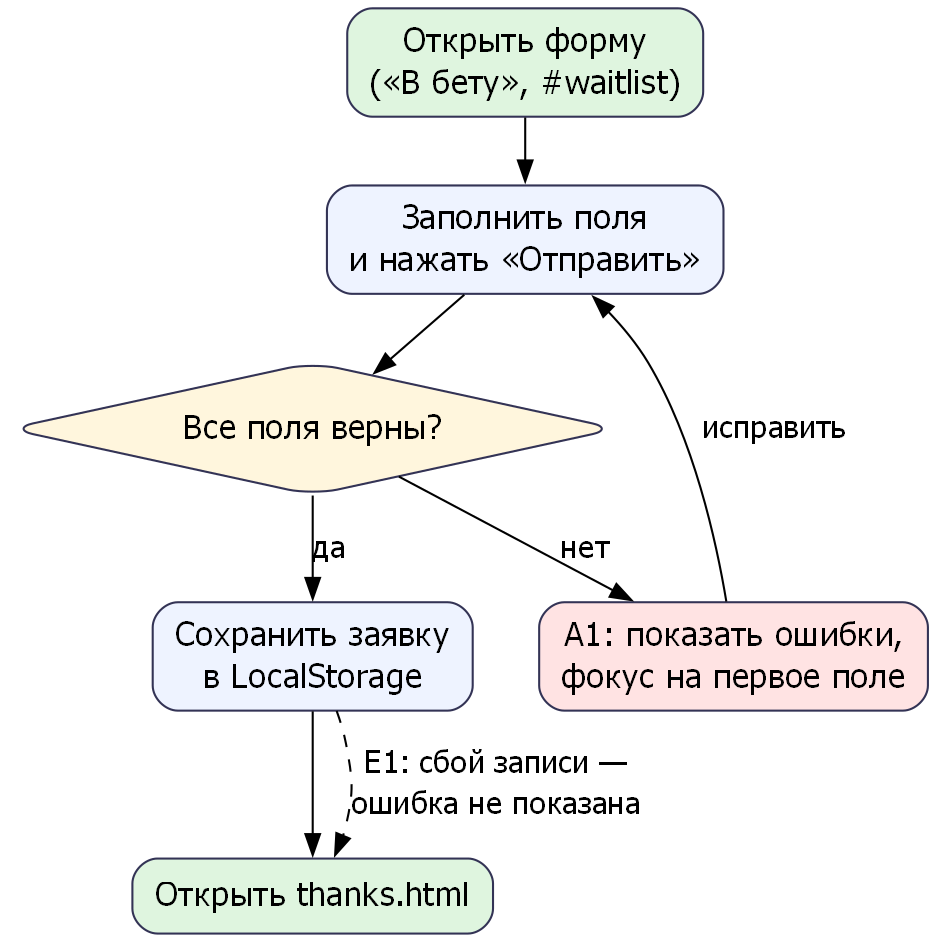
\includegraphics[width=\textwidth,height=0.6\textheight,keepaspectratio]{figures/fig1.png}\par
Рисунок 3.1 – Блок-схема сценария UC-01
\end{center}
\vspace{\baselineskip}

\begin{center}
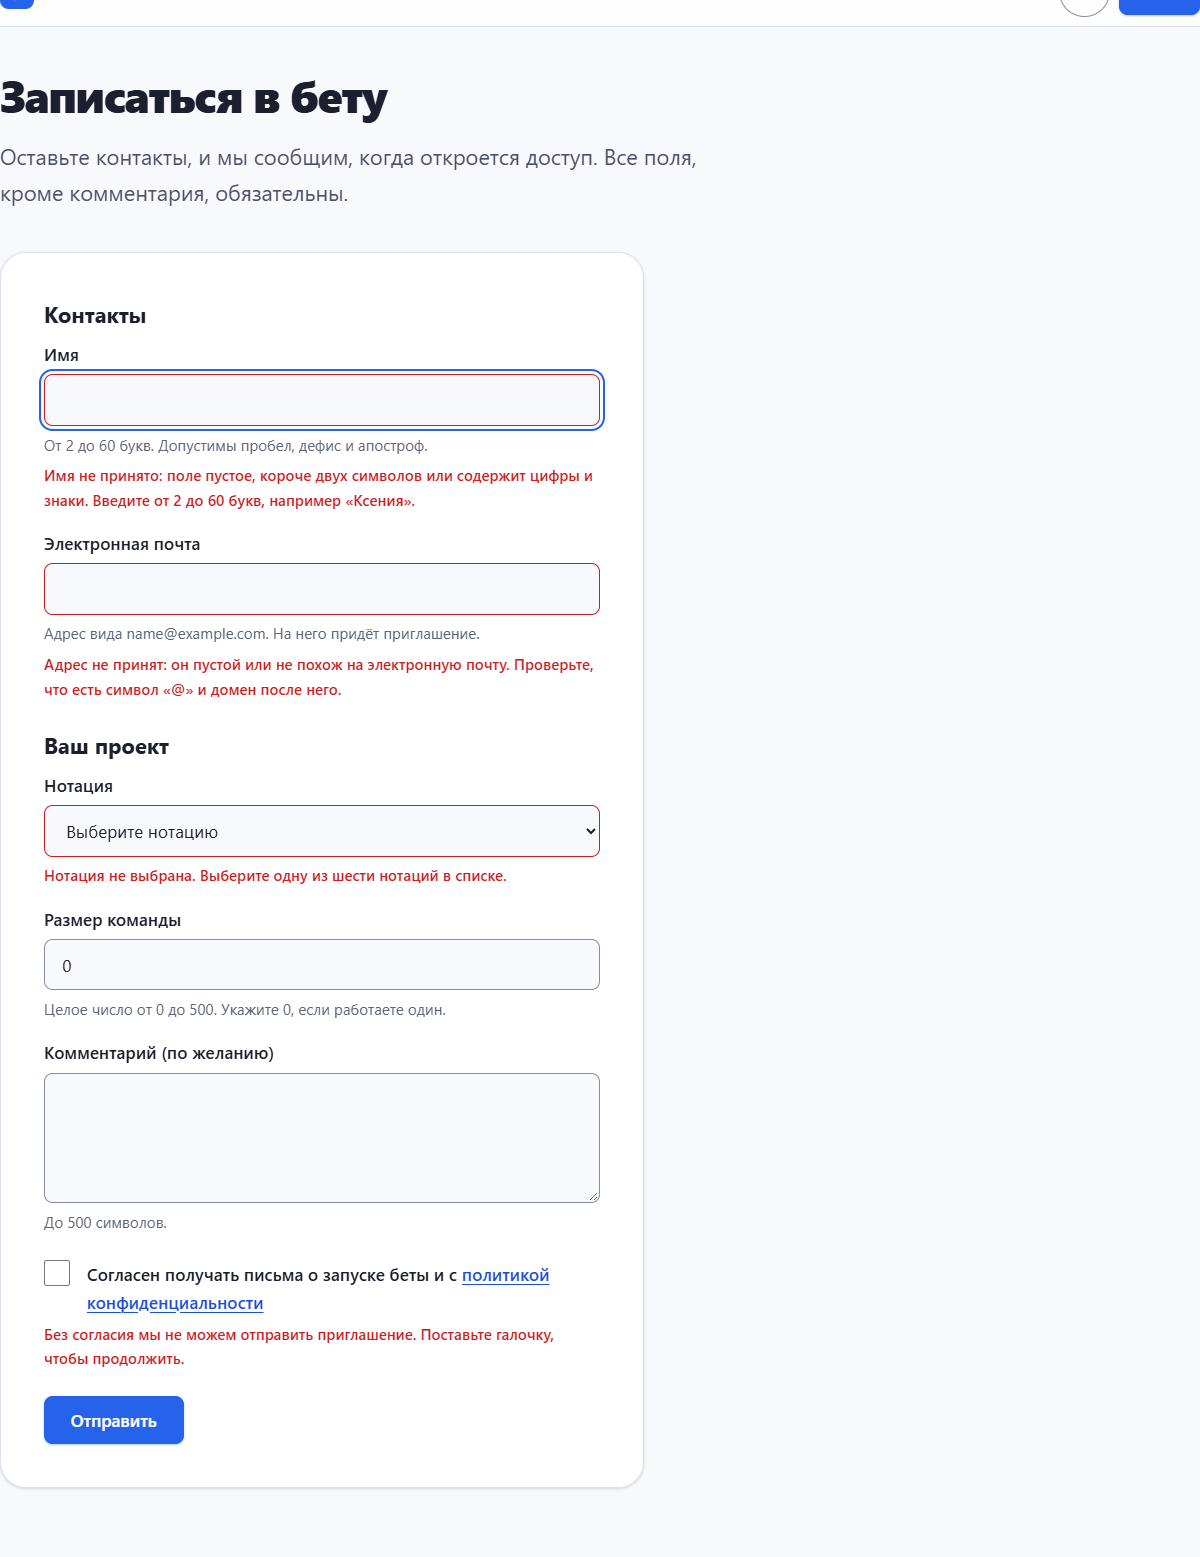
\includegraphics[width=\textwidth,height=0.6\textheight,keepaspectratio]{figures/fig2.png}\par
Рисунок 3.2 – Форма: ошибки при пустой отправке
\end{center}
\vspace{\baselineskip}

\begin{center}
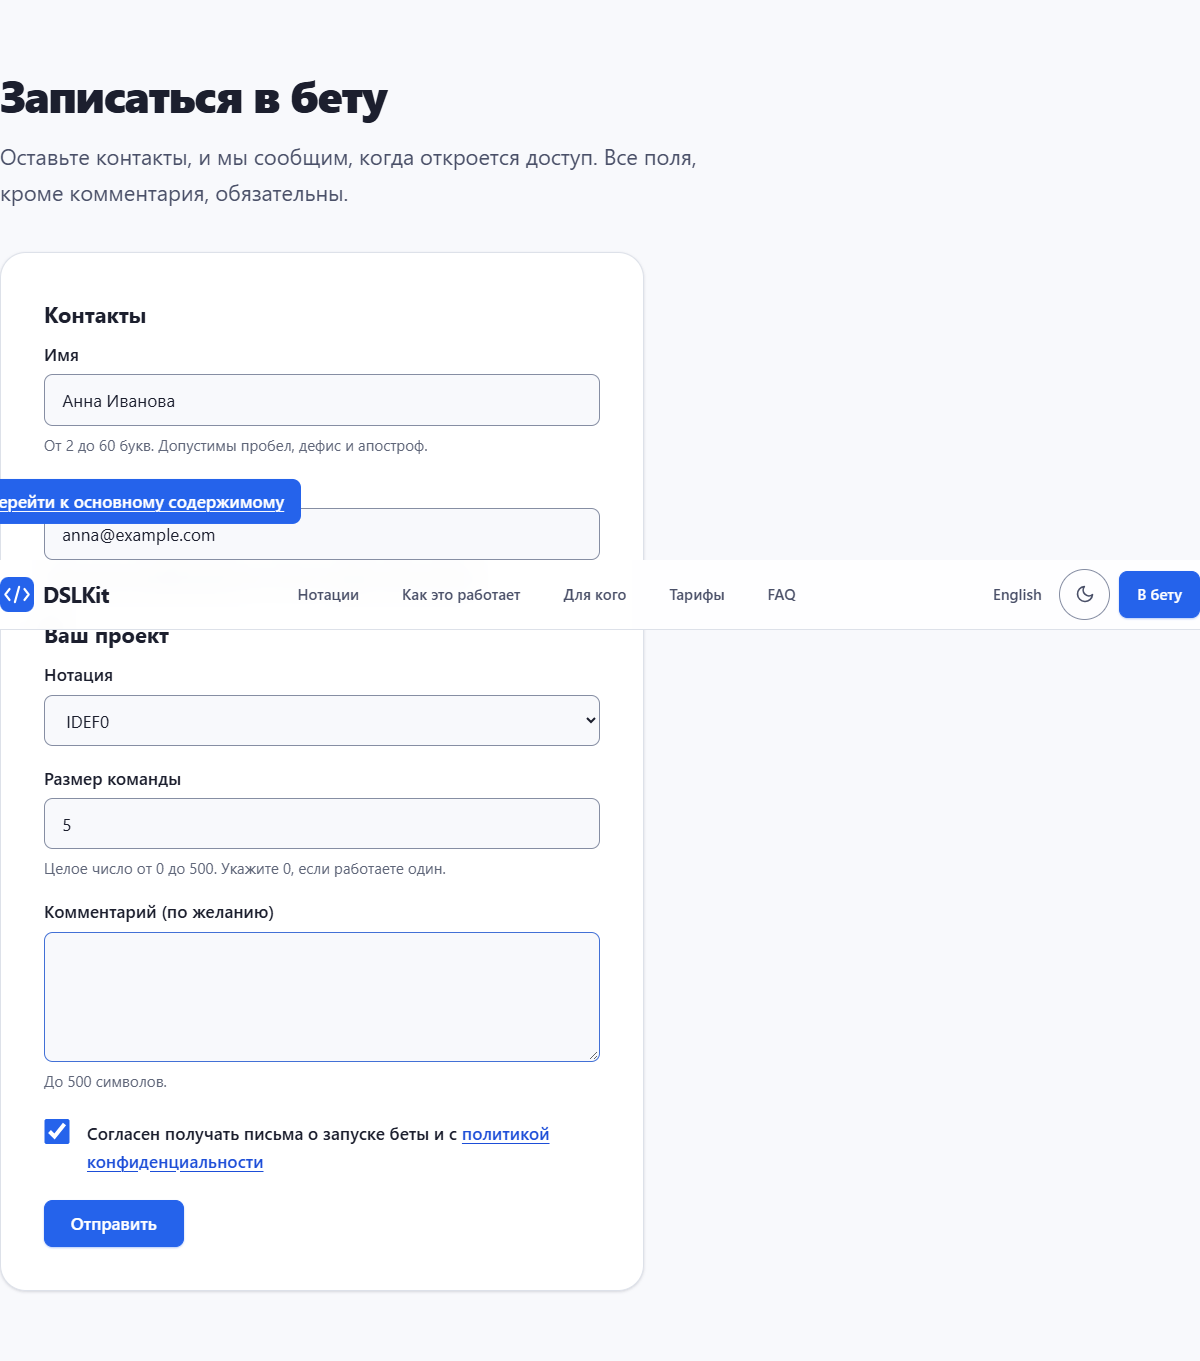
\includegraphics[width=\textwidth,height=0.6\textheight,keepaspectratio]{figures/fig3.png}\par
Рисунок 3.3 – Форма заполнена корректными данными
\end{center}
\vspace{\baselineskip}

\begin{center}
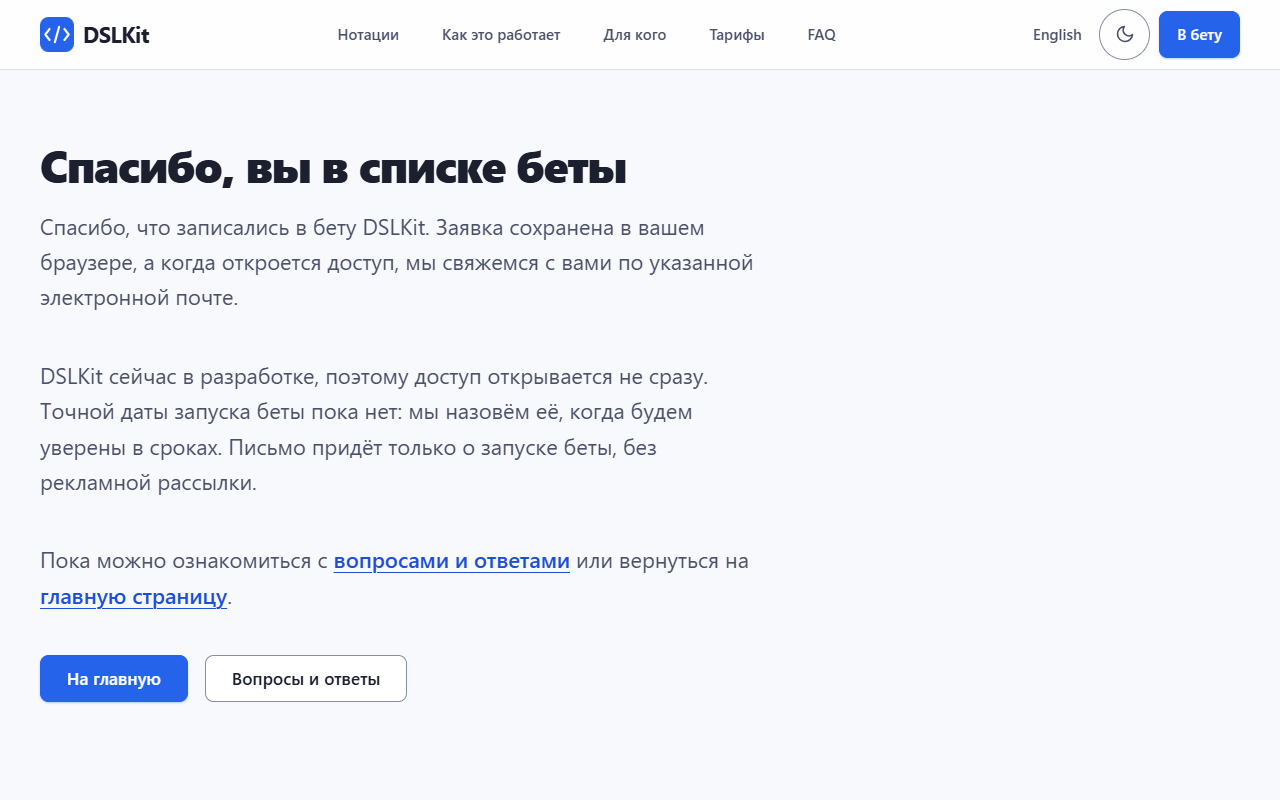
\includegraphics[width=\textwidth,height=0.6\textheight,keepaspectratio]{figures/fig4.png}\par
Рисунок 3.4 – Страница благодарности
\end{center}
\vspace{\baselineskip}

\reportsection{3.3}{Анализ требований и модули}

Тестируется статический сайт DSLKit, запущенный локальным сервером tools/server.js. Требования и модули приведены в таблице ниже.


\noindent Таблица 3.2 – Требования и модули\par\nopagebreak
\begin{longtable}{|>{\raggedright\arraybackslash}p{0.490\textwidth}|>{\raggedright\arraybackslash}p{0.490\textwidth}|}
\hline
ID & Модуль и требование \\ \hline
\endhead
R1 & Доступность страниц (главная, редактор, панель, настройки, английская версия) \\ \hline
R2 & Загрузка стилей и скриптов \\ \hline
R3 & Разбор DSL и преобразование в DOT и Mermaid \\ \hline
R4 & Форма заявки и проверка её полей \\ \hline
R5 & Обработка ошибок сервера: 404, 405, обход каталогов \\ \hline
R6 & Разметка и локализация: lang, h1, title, canonical \\ \hline
R7 & Безопасность: CSP и защитные заголовки \\ \hline
R8 & PWA: манифест, service worker, robots, sitemap \\ \hline
R9 & Локальное хранилище \\ \hline
\end{longtable}
\vspace{\baselineskip}

\reportsection{3.4}{Дымовой чек-лист}

Минимальный набор из 8 проверок. Критический путь запускается только при его успешном прохождении (иначе статус Blocked).


\noindent Таблица 3.3 – Дымовой чек-лист\par\nopagebreak
\begin{longtable}{|>{\raggedright\arraybackslash}p{0.245\textwidth}|>{\raggedright\arraybackslash}p{0.245\textwidth}|>{\raggedright\arraybackslash}p{0.245\textwidth}|>{\raggedright\arraybackslash}p{0.245\textwidth}|}
\hline
ID & Треб. & Проверка & Статус \\ \hline
\endhead
SM-01 & R1 & Главная страница открывается (200) & Passed \\ \hline
SM-02 & R1 & Редактор открывается (200) & Passed \\ \hline
SM-03 & R1 & Панель проектов открывается (200) & Passed \\ \hline
SM-04 & R2 & Стили главной загружаются & Passed \\ \hline
SM-05 & R2 & Скрипт главной загружается & Passed \\ \hline
SM-06 & R3 & Разбор DSL возвращает 2 блока и 1 стрелку & Passed \\ \hline
SM-07 & R4 & Форма заявки есть на главной & Passed \\ \hline
SM-08 & R5 & Несуществующий адрес даёт 404 & Passed \\ \hline
\end{longtable}
\vspace{\baselineskip}

\reportsection{3.5}{Чек-лист критического пути}

36 проверок основных сценариев (таблица ниже).


\noindent Таблица 3.4 – Чек-лист критического пути\par\nopagebreak
\begin{longtable}{|>{\raggedright\arraybackslash}p{0.245\textwidth}|>{\raggedright\arraybackslash}p{0.245\textwidth}|>{\raggedright\arraybackslash}p{0.245\textwidth}|>{\raggedright\arraybackslash}p{0.245\textwidth}|}
\hline
ID & Треб. & Проверка & Статус \\ \hline
\endhead
CP-01 & R1 & Страница / отдаётся как HTML & Passed \\ \hline
CP-02 & R1 & Страница /privacy.html отдаётся как HTML & Passed \\ \hline
CP-03 & R1 & Страница /thanks.html отдаётся как HTML & Passed \\ \hline
CP-04 & R1 & Страница /app/dashboard.html отдаётся как HTML & Passed \\ \hline
CP-05 & R1 & Страница /app/editor.html отдаётся как HTML & Passed \\ \hline
CP-06 & R1 & Страница /app/settings.html отдаётся как HTML & Passed \\ \hline
CP-07 & R1 & Страница /app/welcome.html отдаётся как HTML & Passed \\ \hline
CP-08 & R1 & Страница /en/ отдаётся как HTML & Passed \\ \hline
CP-09 & R1 & Страница /en/privacy.html отдаётся как HTML & Passed \\ \hline
CP-10 & R1 & Страница /en/thanks.html отдаётся как HTML & Passed \\ \hline
CP-11 & R6 & Главная: lang="ru", английская версия: lang="en" & Passed \\ \hline
CP-12 & R6 & На каждой странице ровно один h1 & Passed \\ \hline
CP-13 & R6 & У главной есть canonical и alternate & Passed \\ \hline
CP-14 & R6 & У каждой страницы есть title и meta viewport & Passed \\ \hline
CP-15 & R2 & Все локальные ссылки на ресурсы главной открываются & Passed \\ \hline
CP-16 & R7 & Нет встроенных скриптов (CSP script-src self) & Passed \\ \hline
CP-17 & R7 & Заголовок Content-Security-Policy присутствует & Passed \\ \hline
CP-18 & R7 & X-Frame-Options = DENY & Passed \\ \hline
CP-19 & R7 & X-Content-Type-Options = nosniff & Passed \\ \hline
CP-20 & R5 & POST на статику даёт 405 & Passed \\ \hline
CP-21 & R5 & Выход за корень (../) не отдаёт файлы & Passed \\ \hline
CP-22 & R5 & Страница 404 оформлена как HTML сайта & Passed \\ \hline
CP-23 & R8 & Манифест PWA: корректный JSON с иконками & Passed \\ \hline
CP-24 & R8 & Service worker доступен & Passed \\ \hline
CP-25 & R8 & robots.txt и sitemap.xml доступны & Passed \\ \hline
CP-26 & R3 & parseDsl: тип и заголовок диаграммы & Passed \\ \hline
CP-27 & R3 & parseDsl: порты блока разобраны & Passed \\ \hline
CP-28 & R3 & parseDsl: неизвестная строка попадает в skipped & Passed \\ \hline
CP-29 & R3 & parseDsl: пустой ввод не падает & Passed \\ \hline
CP-30 & R3 & toDot даёт digraph с обоими блоками & Passed \\ \hline
CP-31 & R3 & toMermaid возвращает непустой текст & Passed \\ \hline
CP-32 & R3 & sourceKey: один текст даёт один ключ, разные тексты разные & Passed \\ \hline
CP-33 & R9 & Хранилище: set/get возвращает значение & Passed \\ \hline
CP-34 & R9 & Хранилище: remove и значение по умолчанию & Passed \\ \hline
CP-35 & R4 & Валидация заявки: корректные данные дают пустой список ошибок & Passed \\ \hline
CP-36 & R4 & Форма: у полей есть label и сообщения об ошибках & Passed \\ \hline
\end{longtable}
\vspace{\baselineskip}

\reportchapter{4}{РЕЗУЛЬТАТЫ ТЕСТИРОВАНИЯ}

\reportsection{4.1}{Общая информация}

Проект DSLKit, ветка testing-course, стенд: локальный сервер Node.js, проверки выполнены автоматически командой npm run tc:lab3. Не тестировались: визуальное отображение в браузерах и работа внешнего сервиса Kroki.


\reportsection{4.2}{Метрики}

\noindent Таблица 4.1 – Метрики тестирования\par\nopagebreak
\begin{longtable}{|>{\raggedright\arraybackslash}p{0.327\textwidth}|>{\raggedright\arraybackslash}p{0.327\textwidth}|>{\raggedright\arraybackslash}p{0.327\textwidth}|}
\hline
Метрика & Формула & Значение \\ \hline
\endhead
Выполнено тестов & Выполненные / Всего × 100\% & 100\% \\ \hline
Успешные тесты & Passed / Выполненные × 100\% & 100\% \\ \hline
Плотность дефектов & Дефекты / Количество тестов & 0 \\ \hline
Покрытие требований & Покрытые / Всего × 100\% & 100\% (9 из 9) \\ \hline
\end{longtable}
\vspace{\baselineskip}

Всего проверок 44: Passed 44, Failed 0, Blocked 0.


\reportsection{4.3}{Дефекты, риски и выводы}

Проваленных проверок нет, баг-репорты не требуются. На этапе отладки найдена и исправлена ошибка в самом тестовом наборе (неверный синтаксис DSL во входных данных), продукт при этом работал верно.


Риски: проверки не охватывают отрисовку в браузере и запросы к внешнему сервису диаграмм. Рекомендация: релиз возможен, браузерные сценарии проверять отдельно.


\reportchapter{5}{ВЫВОД}

Составлены дымовой и критический чек-листы, выполнены на стенде, рассчитаны метрики и оформлен отчёт.


\end{document}
